\documentclass[a4paper]{article}

\usepackage{xcolor}
\usepackage{fancyhdr}
\usepackage{listings}
\usepackage{graphicx}
\usepackage[section]{placeins}
\usepackage{hyperref}
\usepackage[utf8]{inputenc}

% colors
\definecolor{mygreen}{rgb}{0,0.6,0}
\definecolor{mygray}{rgb}{0.5,0.5,0.5}
\definecolor{myblue}{rgb}{0,0,0.5}
\definecolor{mymauve}{rgb}{0.58,0,0.82}

% hyperref configuration
\hypersetup{
    colorlinks,
    linkcolor={mymauve},
    citecolor={myblue},
    urlcolor={myblue}
}

% Code listing configuration
\lstset{
  basicstyle=\footnotesize,        % the size of the fonts that are used for the code
  commentstyle=\color{mygreen},    % comment style
  keepspaces=true,                 % keeps spaces in text, useful for keeping indentation of code (possibly needs columns=flexible)
  keywordstyle=\color{blue},       % keyword style
  language=Python,                 % the language of the code
  morekeywords={interface,abstract,static}, % if you want to add more keywords to the set
  %numbers=left,                    % where to put the line-numbers; possible values are (none, left, right)
  numbersep=5pt,                   % how far the line-numbers are from the code
  numberstyle=\tiny\color{mygray}, % the style that is used for the line-numbers
  stringstyle=\color{mymauve}      % string literal style
}

% Translate figure names
\renewcommand{\figurename}{Figuur}

% TODO command
\newcommand{\todo}[1]{\textcolor{red}{[#1]}\\}

% PR command, based on https://tex.stackexchange.com/a/35314/59718
\makeatletter
\newcommand*{\repo}{\begingroup\@makeother\#\@repo}
\newcommand*{\@repo}[2]{%
  \href{https://github.com/DanielSchiavini/design-patterns-assignment/#1}{#2}%
  \endgroup}
\makeatother

\newcommand{\PR}[1]{\repo{pull/#1}{PR\##1}}
\newcommand{\repolink}[1]{\repo{#1}{github.com\-/Daniel\-Schiavini\-/de\-sign-\-pat\-terns-\-as\-sign\-ment\-/#1}}
\newcommand{\cilink}[1]{\href{https://travis-ci.com/DanielSchiavini/design-patterns-assignment/#1}{travis-ci.com/DanielSchiavini/design-patterns-assignment/#1}}

% New custom label command used for requirements, based on https://tex.stackexchange.com/a/18192/59718
% Usage: \customlabel{label}{text}
\makeatletter
\newcommand{\customlabel}[2]{%
   \protected@write \@auxout {}{\string \newlabel {#1}{{#2}{\thepage}{#2}{#1}{}} }%
   \hypertarget{#1}{#2}
}
\makeatother

% new command \requirement{label}{text}
\newcounter{reqcount}
\newcommand{\requirement}[2]{%
  \item \refstepcounter{reqcount}\customlabel{req:#1}{\textbf{Eis \thereqcount}}: #2
}

% New command \reqref{label}
\newcommand{\reqref}[1]{\ref{req:#1}}

% New command \question{text}
\newcommand{\question}[1]{
  \subsection{#1}
}

% New command \code{text}
\newcommand{\code}[1]{\lstinline[columns=fixed]{#1}}

% New command \diagram[width=1.3]{label}{caption}
\newcommand{\diagram}[3][1.3]{
	\begin{figure}[!htb]
	 \caption{#3}
	 \label{diagram:#2}
	 \makebox[\textwidth][c]{\includegraphics[width=#1\textwidth]{Diagrams/#2.pdf}}%
	\end{figure}
}

% heading
\lhead{Open Universiteit}
\chead{IM0102, Design patterns}
\rhead{Eindopdracht}

\begin{document}
\pagestyle{fancy}

\section*{Studentgegevens}
    \begin{description}
        \item [Cursuscode] IM0102
        \item [Opdracht] Jabberpoint Inhoudsopgave
        \item [Naam] Daniel S. C. Schiavini
        \item [Studentnummer] 851102873
    \end{description}

\section*{Aanpak}
    \label{sec:aanpak}
	De eerste versie van deze opdracht is afgekeurd doordat de opdracht niet goed begrepen was.
	De refactoring was niet compleet doorgevoerd, maar alleen in de onderdelen die nodig waren om de inhoudsopgave toe te voegen.
	Deze sectie is daarom verdeeld tussen de eerste versie en de volledige refactoring.

	\subsection*{Eerste versie}
    De oorspronkelijke bedoeling was om deze opdracht uit te voeren in een team met een andere student.
    Echter, er was geen andere student beschikbaar met een vergelijkbare tempo.
    Daardoor heb ik deze opdracht alleen uitgevoerd.

    Voordat ik wist dat ik de opdracht alleen mocht uitvoeren, had ik al een Git repository gemaakt.
    Ik heb de repository zo geconfigureerd dat dit document automatisch wordt gebouwd door het gebruik van TravisCI.
    Zodra een nieuwe versie van het rapport naar GitHub wordt gepushed, draait een script dat het PDF-bestand maakt.
    Het script bouwt ook Jabberpoint, draait unit tests, en als alles gelukt is wordt ook een JAR-bestand gemaakt.
    In de master branch hangt een deployment vast dat het PDF en JAR naar \href{https://github.com/DanielSchiavini/design-patterns-assignment/tree/gh-pages}{GitHub pages} publiceert.
    Deze automatisering is iets minder nodig zonder team, maar het is nog steeds wel nuttig.
    De CI-configuratie is beschikbaar op \repolink{blob/master/.travis.yml}.

    Jabberpoint had nog geen geautomatiseerde tests en omdat ik dat belangrijk vind, heb ik van tevoren JUnit tests geschreven (zie \PR{5}, \PR{9} en \PR{10}).
    Echter niet alle klassen waren testbaar -- TravisCI draait in een Linux-container waarin de Graphic Java-klassen niet gecreëerd kunnen worden.
    Ik had niet genoeg tijd had om dit probleem op te lossen, daarom heb ik alleen tests geschreven voor de domein- en accessor-klassen.
    Het probleem van UI-domein vermenging wordt verder besproken in sectie~\ref{q:ui-domein-vermenging}.

    Het schrijven van de tests was een goede hulpmiddel om Jabberpoint te leren kennen en om het probleemanalyse van de volgende sectie beter uit te voeren.
	De tests zijn hierbij erg waardevol geweest tijdens de refactoring.
	In vrijwel alle gevallen, als de tests sloegen werkte de applicatie via de gebruikersinterface ook.

	\subsection*{Volledige refactoring}
	In de nieuwe versie van Jabberpoint heb ik de applicatie opnieuw gestructureerd.
	Ten eerste is de applicatie verdeeld tussen model, view en controller (MVC patroon).
	Vervolgens heb ik alle onderdelen doorgenomen en steeds verbeteringen doorgevoerd, met de volgende regels in gedachte:
	\begin{itemize}
		\item Elk klasse moet precies één verantwoordelijkheid hebben.
		\item Elke methode moet precies één verantwoordelijkheid hebben.
		\item Delegatie liever dan overerving.
		\item Geen constructor-aanroepen buiten factories.
		\item Alles wat een klasse nodig heeft om te functioneren wordt in de constructor meegegeven.
	\end{itemize}

	De details over het resultaat van de refactoring worden belicht in de volgende secties.
	\todo{MVC Diagram}

\section{Probleemanalyse}
    \label{sec:probleemanalyse}

	\subsection{Inhoudsopgave}
    Om de inhoudsopgave te analyseren kunnen we het beste de opdracht in eisen omschrijven:

    \begin{itemize}
        \requirement{toevoegen}{De gebruiker moet één of meer slides met inhoudsopgaven kunnen toevoegen aan een presentatie.}
        \requirement{tonen}{Een inhoudsopgave-slide moet alle onderwerpen van de presentatie tonen.}
        \requirement{samenvoegen}{Het onderwerp moet slechts eenmaal worden getoond wanneer meerdere slides achter elkaar hetzelfde onderwerp hebben.}
        \requirement{updaten}{De inhoudsopgave moet automatisch worden geüpdatet wanneer slides worden toegevoegd of verwijderd.}
        \requirement{titel}{De titel moet als onderwerp worden gebruikt wanneer een slide geen onderwerp heeft (\textbf{aanname}).}
        \requirement{onderwerpen}{Het onderwerp mag op slides worden getoond, behalve in de inhoudsopgave (optioneel).}
        \requirement{volgnummers}{De onderwerpen in de inhoudsopgave mogen volgnummers krijgen (optioneel).}
        \requirement{aanduiding}{Het onderwerp van de slide die na een inhoudsopgave komt, mag een speciale aanduiding krijgen (i.e. een alternatieve letterstijl) (optioneel).}
        \requirement{stijl}{De stijl van de inhoudsopgave is vrij te bepalen.}
    \end{itemize}

    De opdracht om een inhoudsopgave te implementeren in Jabberpoint is best interessant.
    Om een inhoudsopgave te tonen, is kennis nodig van de hele presentatie.
    Een verandering in elke slide kan invloed hebben op alle inhoudsopgaven.
    Deze circulaire afhankelijkheid maakt de opdracht uitdagend.

	\subsection{Refactoring}
	In de eerste fase van de opdracht zijn een aantal problemen geconstateerd:
	\begin{itemize}
		\item De applicatie had geen duidelijke scheiding tussen gebruikersinterface en business-logica.
			Om dit op te lossen is de MVC-patroon gebruikt.
		\item AWT-afhankelijkheden waren verspreid door de code.
			Hierdoor was het moeilijk om nieuwe gebruikersinterfaces te maken en om de applicatie te testen.
		\item Instanties werden in verschillende locaties gemaakt en vaak werd de klasse pas bruikbaar na andere methode-aanroepen.
			Het was bijvoorbeeld mogelijk om een \code{TextItem} te maken zonder tekst.
		\item De Java-versie was verouderd geworden.
	\end{itemize}

\section{Ontwerp}
    \label{sec:ontwerp}
	De applicatie is nu gesplitst in meerdere Java-packages die volgen het MVC-patroon.
	In de onderstaande secties worden de verschillende packages belicht.

	\subsection{Jabberpoint}
		In de package \code{jabberPoint} vinden we de \code{Jabberpoint} klasse, die verantwoordelijk is om alle afhankelijkheden aan elkaar te verbinden.
		Hierdoor kan de hele applicatie werken zonder dat instanties buiten factories worden gemaakt (\textit{Depedency Injection} patroon).
		Deze klasse heeft een \code{main} methode die een presentatie opent door middel van de gemaakte factories.

	\subsection{Model}
		Het \code{jabberPoint.model} package bevat alle business-logica en is nu helemaal onafhankelijk van de gebruikersinterface.
		Het klassendiagram wordt in figuur~\ref{diagram:model} getoond.

		\diagram{model}{
			Klassendiagram voor de model-klassen.
			Factories zijn weggelaten.
			Referenties naar controller en view zijn beperkt gehouden voor de duidelijkheid.
			Het \code{utils} package wordt in grijs getoond.
		}

		De \code{Presentation}-klasse is duidelijk centraal in het systeem.
		Een presentatie heeft meerdere slides, en slides kunnen inhoud of inhoudsopgave bevatten.
		Slides kunnen meerdere slide-items bevatten, welke plaatjes of tekst mogen zijn.
		Samen met de stylen is de presentatie-datastructuur compleet.

		Deze data-klassen mogen niets weten van de gebruikersinterface waarin ze worden getoond.
		Wel zijn deze klassen verantwoordelijk om de gegevens op een generieke manieren te converteren.
		In dit geval was het vanzelfsprekend om een XML-formaat te gebruiken, maar dit had ook JSON kunnen zijn.

		Naast de data-klassen hebben we de I/O klassen voor het lezen en schrijven van presentaties.
		Het lezen van presentaties kan op twee manieren gebeuren: vanuit een file of vanuit een demo-presentatie.
		De presentatie kan ook naar een bestand worden geschreven.
		De klasse verantwoordelijk daarvoor is veel simpeler geworden doordat deze geen kennis hoeft te hebben van de datastructuur.

		Om te voorkomen dat de presentatie iets weet van de gebruikersinterface maar toch deze kan updaten, heb ik ervoor gekozen om het \textit{Observable-patroon} te implementeren.
		De Java-klassen hiervoor hebben geen typing, waardoor casts nodig zijn.
		Door de toepassing van generics kan dit verbeterd worden.
		Daarom heb ik het patroon geïmplementeerd door middel van twee interfaces en één abstracte klasse.
		Op deze manier kan de presentatie een \code{BaseObservable<Slide>} uitbreiden en \textit{observers} laten weten als een nieuwe slide moet worden getoond.
		De \textit{observable}-klassen zijn gegroepeerd in het package \code{utils} omdat ze niet specifiek voor Jabberpoint zijn.

		\subsubsection{Factories}
			Alle klassen mogen alleen door factories worden gemaakt.
			Deze factories worden gegroepeerd in het package \code{jabberPoint.model.factories}.
			Een klassendiagram van dit package wordt in figuur~\ref{diagram:model-factories} getoond.

			\diagram{model-factories}{
				Klassendiagram voor de model-factories.
				Details zijn weggelaten voor de duidelijkheid.
			}

		\subsubsection{Inhoudsopgave}
			De oude klasse \code{Slide} is nu gesplitst in een abstracte klasse \code{Slide} en de sub-klasse \code{ContentSlide}.
			De nieuwe klasse \code{TableOfContentsSlide} genereert de inhoudsopgaven.

			De grootste verschillen tussen de subklassen zijn dat de inhoudsopgave kennis moet hebben van de hele presentatie en zijn eigen inhoud moet genereren.
			Daardoor krijgt een \code{TableOfContentsSlide} een referentie naar de presentatie in de constructor.

			De \code{Slide} klasse heeft nu een \code{getSlideItems} abstracte methode.
			Voor de normale slides zijn de slide items aanpasbaar, voor de inhoudsopgave worden de items gegenereerd.
			Omdat er geen speciale stijl-eisen zijn voor de inhoudsopgave, kunnen wij eenvoudig de al ingebouwde levels gebruiken om de stijl te bepalen.
			De views hoeven dus ook niet te weten wat voor soort slide getoond wordt.

			Een screenshot van de inhoudsopgave van de demo-presentatie wordt in figuur~\ref{fig:master} getoond.
			\begin{figure}[!htb]
			 \caption{
				Inhoudsopgave van de demo-presentatie.\label{fig:master}
			 }
			 \centering 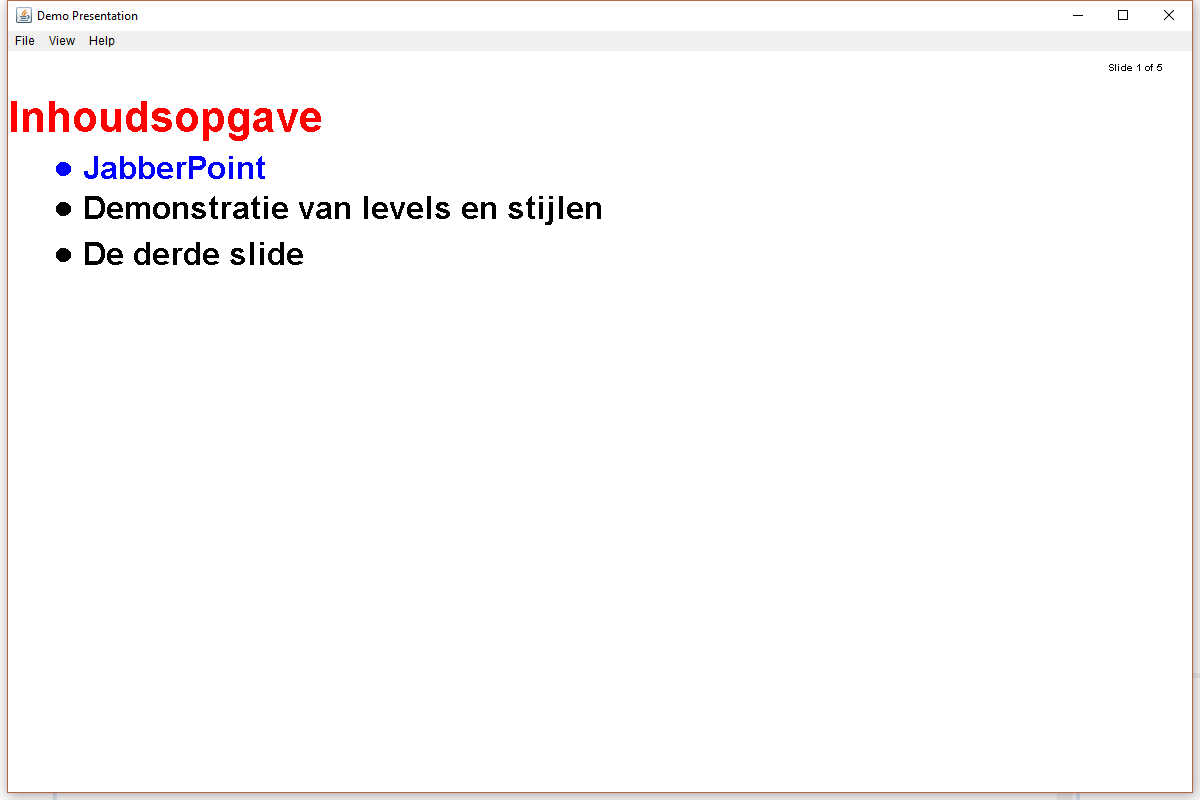
\includegraphics[width=\textwidth]{Screenshots/master.png}
			\end{figure}

		\subsubsection{Traceerbaarheid van eisen}
			In deze sectie geef ik onderdelen van het ontwerp aan die verantwoordelijk zijn om de eisen (zie sectie~\ref{sec:probleemanalyse}) te realiseren.
			Dit geeft dus de relatie tussen probleemanalyse en ontwerp.

			\begin{itemize}
				\item De \code{Accessor}-klassen zijn verantwoordelijk voor \reqref{toevoegen}.
				\item De \code{TableOfContentsSlide} klasse is verantwoordelijk voor \reqref{tonen}, \reqref{samenvoegen},
					\reqref{updaten}, \reqref{titel}, \reqref{volgnummers}, \reqref{aanduiding} en \reqref{stijl}.
				\item De \code{Slide} klasse is verantwoordelijk voor \reqref{onderwerpen}.
			\end{itemize}

	\subsection{View}\label{sec:view}
		Het \code{jabberPoint.view} package bevat alle nodige code voor de gebruikersinterface.
		Het element dat het volledige scherm opbouwt is de \code{JabberpointFrame}.
		Deze klasse bevat de twee controllers (zie sectie~\ref{sec:controller}) en de \code{PresentationView}.

		\code{PresentationView} krijgt de presentatie als referentie en is verantwoordelijk om de juiste slide te tonen.
		Om te weten wanneer een nieuwe slide moet worden getoond maak ik gebruik van het \textit{observable-patroon}.
		Op het moment dat de \code{update} methode wordt aangeroepen, wordt een nieuwe \code{SlideView} gemaakt via de bijbehorende factory.

		De \code{SlideView} klasse is verantwoordelijk om de slide te tekenen, inclusief de \code{SlideItemView} instanties.
		Deze kunnen of een \code{BitmapItemView} of een \code{TextItemView}, maar de keuze voor de juiste view gebeurt ook in de factory (zie sectie~\ref{sec:view-factories})

		Het klassendiagram van de view wordt in figuur~\ref{diagram:view} getoond.

		\diagram[1]{view}{
			Klassendiagram voor de view-klassen.
			Factories zijn weggelaten.
			Referenties naar controller en model zijn beperkt gehouden voor de duidelijkheid.
		}
		
		\subsubsection{Factories}\label{sec:view-factories}
			Alle klassen mogen alleen door factories worden gemaakt.
			Deze factories worden gegroepeerd in het package \code{jabberPoint.view.factories}.
			Een klassendiagram van dit package wordt in figuur~\ref{diagram:view-factories} getoond.

			\begin{figure}[!htb]
			 \caption{
				Klassendiagram voor de view-factories.\label{diagram:view-factories}
				Details zijn weggelaten voor de duide\-lijk\-heid.
			 }
			 \todo{factory diagram} % \makebox[\textwidth][c]{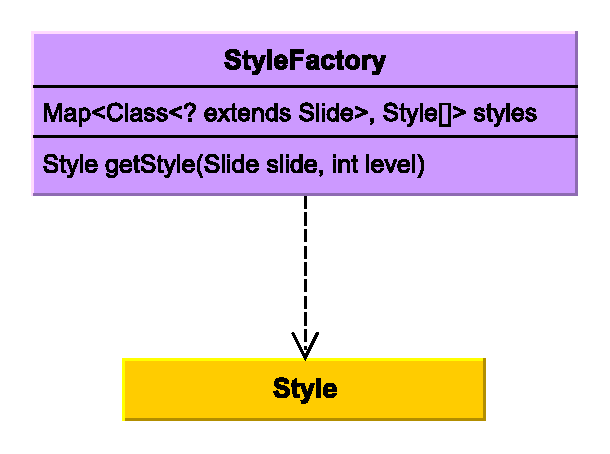
\includegraphics[width=1.3\textwidth]{Diagrams/view-factories.pdf}}%
			\end{figure}

	\subsection{Controller}\label{sec:controller}
		Het \code{jabberPoint.controller} package bevat alle nodige code voor het veranderen van de model via de gebruikersinterface.
		Jabberpoint kent twee manieren om de presentatie te navigeren: via de menu of via het toetsenbord.
		Daarom hebben we ook twee controllers: \code{MenuController} en \code{KeyController}.
		Het klassendiagram wordt in figuur~\ref{diagram:controller} getoond.

		\begin{figure}[!htb]
		 \caption{
			Klassendiagram voor de controller-klassen.\label{diagram:controller}
			Factories zijn weggelaten.
			Referenties naar view en model zijn beperkt gehouden voor de duidelijkheid.
		 }
		 \todo{diagram} % \makebox[\textwidth][c]{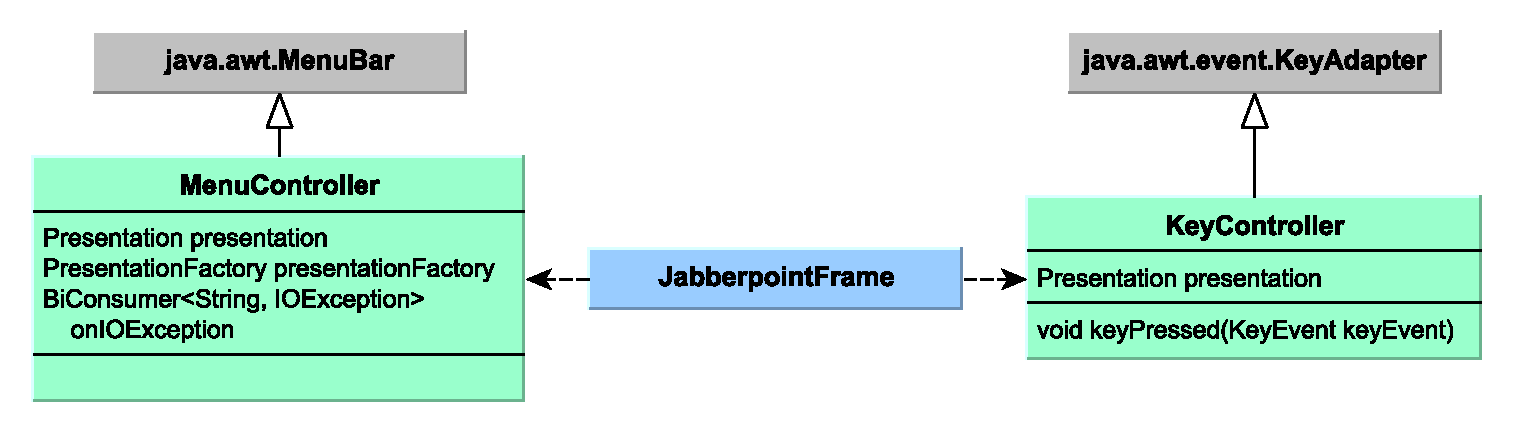
\includegraphics[width=1.3\textwidth]{Diagrams/controller.pdf}}%
		\end{figure}

		\subsubsection{Factories}
			Alle klassen mogen alleen door factories worden gemaakt.
			Deze factories worden gegroepeerd in het package \code{jabberPoint.controller.factories}.
			Een klassendiagram van dit package wordt in figuur~\ref{diagram:controller-factories} getoond.

			\begin{figure}[!htb]
			 \caption{
				Klassendiagram voor de controller-factories.\label{diagram:controller-factories}
				Details zijn weggelaten voor de duide\-lijk\-heid.
			 }
			 \todo{factory diagram} % \makebox[\textwidth][c]{
\includegraphics[width=1.3\textwidth]{Diagrams/controller-factories.pdf}}%
			\end{figure}


\section{Keuzen}\label{sec:keuzen}
    In deze sectie gaan we een aantal vragen door die zijn opgeroepen tijdens het analyseproces.
   
    \question{Welke klasse is verantwoordelijk voor onderwerpen?}
		De inhoudsopgave moet toegang krijgen tot een lijst van onderwerpen in de presentatie.
		In het ontwerp krijgt \code{TableOfContentsSlide} een referentie naar de presentatie en is zelf verantwoordelijk om deze te lezen.
		En alternatief hierop is om de presentatie verantwoordelijk te houden voor de onderwerpen in de slides.
		\code{TableOfContentsSlide} zou dan een dan een onderwerpen-lijst ontvangen.

		De voordelen van deze alternatief zijn:
		\begin{itemize}
			\item De inhoudsopgave hoeft niets te weten van de presentaties.
			\item De presentatie is verantwoordelijk om zijn eigen slides te lezen.
			\item De circulaire referentie wordt opgeheven.
			\item De lijst van onderwerpen kan tussen de verschillende inhoudsopgaven worden gedeeld.
		\end{itemize}

		De nadelen zijn:
		\begin{itemize}
			\item Er komt meer logica in de presentatie die alleen nodig is voor de in\-houds\-op\-gave.
			\item De inhoudsopgaven moeten nog steeds alle items doorlopen om te bepalen welk onderwerp het volgende is.
			\item De methoden die nodig zijn om de slides te lezen bestaan al in de presentatie.
			\item Het is conceptueel correct om een circulaire referentie te hebben, immers een inhoudsopgave moet een overzicht van de presentatie laten zien.
			\item De presentatie klasse wordt nog complexer.
		\end{itemize}

		De keuze om de lijst van onderwerpen in de inhoudsopgave te implementeren geeft dus een betere inkapseling.

    \question{Moet een inhoudsopgave verplicht een titel hebben?}
		In de opdracht wordt niet benoemd of elke inhoudsopgave verplicht een titel moet krijgen.
		De opgeleverde versie van de applicatie geeft een standaard-titel (``inhoudsopgave'') als er geen titel wordt gegeven.
		Echter aangezien alle slides een titel nodig hebben, is het niet raar om de titel van de inhoudsopgave ook verplicht te maken.
		Deze aanpassing is geïmplementeerd in \PR{21}.
    
    \question{Moet een inhoudsopgave een andere stijl krijgen?}
		De standaard stijl van de slides is niet optimaal voor een inhoudsopgave, alhoewel \reqref{stijl} expliciet aangeeft dat stijlen vrij te bepalen zijn.
		Het is echter niet helemaal duidelijk dat het om een lijst van onderwerpen gaat.
		Door een icoontje of nummer toe te voegen aan elke item en steeds dezelfde indentatie te gebruiken, wordt het duidelijker.
		Een screenshot van de inhoudsopgave met deze stijl wordt in figuur~\ref{fig:master} getoond.

    \question{Moet de versiegeschiedenis in de bestanden zijn?}
		In de initiële versie van Jabberpoint stond bovenaan in elk bestand een geschiedenis van de versies.
		Met een moderne ontwikkelmethode verandert de code heel snel, de lijst wordt heel lang en niet altijd up-to-date gehouden.
		Bovendien gebruiken we nu een tool die specifiek gemaakt is om code-geschiedenis bij de houden, namelijk Git.
		Daarom heb ik besloten om deze versiegeschiedenis te verwijderen van alle files en deze alleen in Git te houden.

    \question{Moet de code worden voorzien van Javadoc?}
		Om software echt onderhoudbaar te maken is het ontwikkelen met ontwerp-patronen niet voldoende.
		Ik ben namelijk van mening dat de documentatie bij de code van essentieel belang is.
		Daarnaast is het schrijven van de bedoeling van een stukje code een belangrijk hulpmiddel om de codekwaliteit te evalueren.
		Daarom heb ik de hele applicatie voorzien van Javadoc op het niveau van klassen en methoden.
		De meeste attributen zijn overigens ook gedocumenteerd.

	\question{Is het updaten van Java verstandig?}
		De Jabberpoint applicatie maakte gebruik van Java 1.6.
		Tijdens de refactoring heb ik besloten om de Java-versie te updaten naar 1.8.
		Met deze versie van Java is het gebruik van lambda-functies mogelijk.
		Daardoor was het mogelijk om de controllers veel eenvoudiger te maken.

\section{Sourcecode}
	In deze sectie geef ik links naar de verschillende resultaten van de opdracht.
	Alle links betreffen zowel Jabberpoint als dit rapport.
	\begin{itemize}
		\item Jabberpoint code:
			\repolink{tree/master/Jabberpoint}\\
			De werking ervan wordt uitgelegd in sectie~\ref{sec:ontwerp}.
		\item \LaTeX ~code:
			\repo{tree/master/Report}{github.com/DanielSchiavini/design-patterns-assignment/tree\-/master\-/Report}
		\item Aanpassingen op Jabberpoint:
			\repolink{compare/v0.0.1...master}.
		\item Gegenereerde bestanden:
			\repolink{tree/gh-pages}
		\item Laatste build-rapport van TravisCI:
			\cilink{}
		\item Rapporten van TravisCI:
			\cilink{builds}
		\item Optionele implementaties:
			\repolink{pulls}
	\end{itemize}

\end{document}
